% 2008 年湖南卷理科第 17 题：四棱锥 P-ABCD，底面 ABCD 是边长 1 的菱形，∠BCD=60°，
%   E 是 CD 的中点，PA ⊥ 底面，PA=2。
% 来源 PDF：gaokaomath-src/普通高考/2008/2008湖南理.pdf
% SHA-256：a702a9a7fbdfa2d31961e21e2da7a555ce4ad67771f88fa28c9f99d659b913d7
% 原页：2008湖南理.pdf 第 1 页（A3 三栏）第 3 栏，书页码 453。
% 绘制依据：底面取斜投影 (x,y)->(x+0.5y, 0.55y)，正三角形 ABD 与 BCD 共边；
%   A(0,0)、B(1,0)、D(0.5,0.866)、C(1.5,0.866)，P 在 A 的正上方（高 2），E 为 CD 中点。
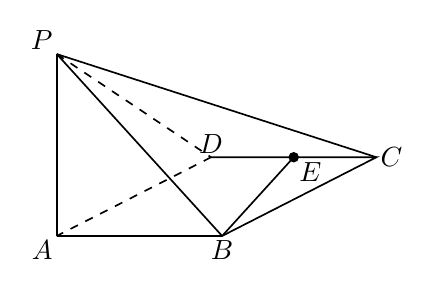
\begin{tikzpicture}[scale=2.1, semithick, every node/.style={inner sep=1.2pt}]
  \coordinate (A) at (0.00,0.00);
  \coordinate (B) at (1.00,0.00);
  \coordinate (D) at (0.933,0.476);
  \coordinate (C) at (1.933,0.476);
  \coordinate (P) at (0.00,1.10);
  \coordinate (E) at (1.433,0.476);

  % 底面
  \draw (A) -- (B) -- (C) -- (D);
  \draw[dashed] (D) -- (A);

  % 侧棱
  \draw (P) -- (A);
  \draw (P) -- (B);
  \draw (P) -- (C);
  \draw[dashed] (P) -- (D);

  % BE
  \draw (B) -- (E);

  \fill (E) circle (0.9pt);

  \node[below left] at (A) {$A$};
  \node[below] at (B) {$B$};
  \node[right] at (C) {$C$};
  \node[above] at (D) {$D$};
  \node[above left] at (P) {$P$};
  \node[below right=0.5pt] at (E) {$E$};
\end{tikzpicture}
